\documentclass[10pt]{article}
\usepackage{icmlko}

\icmlmeta{IP 파운데이션 월드모델}{170}{걸음을 바꿔도 부호가 그대로인가}{한 칸이 얼마인지 못 정하겠으면 다섯 가지로 다 재 보면 된다. 부호가 안 바뀌는 칸만 믿으면 되고, 그 표지가 라벨도 사전 부호도 안 본다}

\begin{document}

\twocolumn[
\icmlheader

\begin{abstract}
노트 169가 섭동 크기를 고정 0.25에서 관측 간격으로 고치자 축별 크기 순위가
바뀌고 노트 163의 설명이 무너지는 것을 보이고, ``고정과 간격 중 무엇이
손잡이의 뜻인가''를 남겼다. \textbf{고르는 대신 다섯을 다 재기로 했다} ---
0.05 · 0.10 · 0.25 · 0.50 · 관측 간격. 그리고 \textbf{다섯에서 부호가
그대로인 칸만 믿는다.} 이 표지는 라벨도 사전 부호도 안 보고 매겨지므로
순환이 아니다. 결과가 셋이다. \textbf{① 되는 축은 전 칸이 불변이다} ---
타깃 폭 9/9, 굿즈 규모 8/8이 두 정식화 모두다. 반대로 F18 배깅에서 장소
노출은 3/7, 입장 마찰은 5/8밖에 안 된다. 노트 163부터 여섯 노트가 지목해
온 그 둘이다. \textbf{② 표지가 정확도를 가른다} --- F18 에서 걸음 불변 칸의
사전 부호 정확도가 \textbf{26/28 = 93\%}이고 흔들리는 칸은 \textbf{5/8 =
62\%}다. 31\%p 차이다. \textbf{③ 트리가 더 흔들린다} --- F18 배깅은 28/36
= 78\%가 불변인데 F6 능형은 \textbf{35/36 = 97\%}다. 조각별 상수인 모형은
걸음이 분기를 넘느냐에 따라 답이 달라지고, 선형은 걸음에 비례할 뿐이라
부호가 안 바뀐다. \textbf{판 1위가 걸음에 흔들리고 판 4위가 안 흔들린다}
--- 노트 156부터 이어진 ``판을 잘 맞힐수록 손잡이를 못 돌린다''가 또
같은 방향이다. \texttt{lab/lever.py} 에 \texttt{stable} ·
\texttt{stable\_acc} 로 넣고 실행 요약에 싣는다. \textbf{노트 169가 남긴
``한 칸을 못 정하겠다''는 문제가 풀린 것은 아니다} --- 다만 못 정해도
쓸 수 있는 칸을 고를 수는 있게 됐다.
\end{abstract}
]

\begin{figure*}[t]
\centering
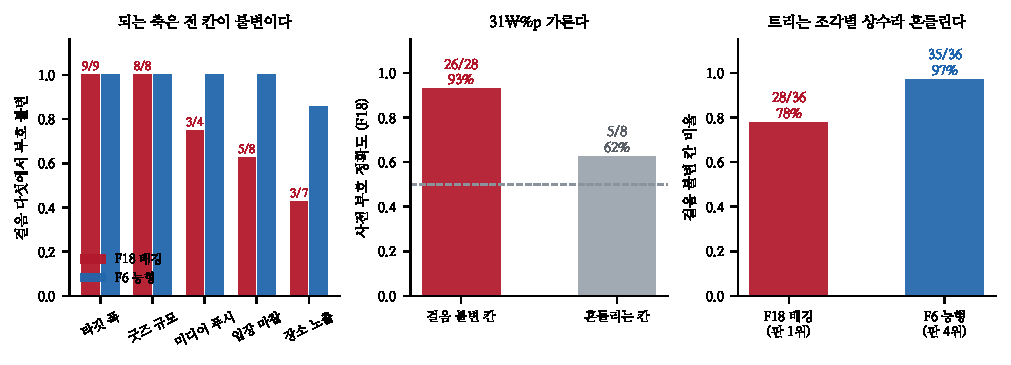
\includegraphics[width=\textwidth]{figs/stable.pdf}
\caption{왼쪽 --- 되는 축은 전 칸이 불변이다. 가운데 --- 표지가 31\%p
가른다. 오른쪽 --- 트리가 더 흔들린다.}
\end{figure*}

\section{고르는 대신 다섯을 다 잰다}

\begin{table}[t]
\centering\tsize
\caption{걸음 다섯에서 부호가 그대로인 칸.}
\begin{tabular}{lrr}
\toprule
& F18 배깅 & F6 능형 \\
\midrule
\textbf{타깃 폭} & \textbf{9/9} & \textbf{9/9} \\
\textbf{굿즈 규모} & \textbf{8/8} & \textbf{8/8} \\
미디어 푸시 & 3/4 & 4/4 \\
입장 마찰 & 5/8 & 8/8 \\
장소 노출 & \textbf{3/7} & 6/7 \\
\midrule
합 & 28/36 & \textbf{35/36} \\
\bottomrule
\end{tabular}
\end{table}

\claimx{\textbf{되는 축은 전 칸이 불변이다.} 타깃 폭 9/9 · 굿즈 규모 8/8이
두 정식화 모두다. 노트 163부터 여섯 노트가 ``이 둘만 손잡이''라고 해 온
그 둘인데, \textbf{이번 표지는 사전 부호를 안 보고 매긴 것}이다.}{독립적인
증거라는 뜻이다 --- 앞의 여섯 노트는 전부 ``내 상식과 맞나''를 봤고 이건
``걸음을 바꿔도 답이 같나''만 본다.}

\section{표지가 정확도를 가른다}

\begin{table}[t]
\centering\tsize
\caption{F18 배깅. 걸음 0.25에서의 부호로 채점.}
\begin{tabular}{lrr}
\toprule
& 칸 & 사전 부호 정확 \\
\midrule
\textbf{걸음 불변} & 28 & \textbf{26/28 = 93\%} \\
흔들림 & 8 & 5/8 = 62\% \\
\bottomrule
\end{tabular}
\end{table}

\claimx{\textbf{31\%p 가른다.} 불변 칸은 93\%, 흔들리는 칸은 62\%로 동전
근처다. 그러니 흔들리는 칸의 손잡이 읽기는 쓰지 않는 것이 맞다.}{F6 능형은
흔들리는 칸이 하나뿐이라(아이돌 · 장소 노출) 같은 대조를 못 한다.
\textbf{표지가 쓸모 있으려면 흔들리는 칸이 어느 정도 있어야 하는데, 그
자체가 그 모형이 덜 미덥다는 뜻이다.}}

\section{트리가 더 흔들린다}

\claimx{\textbf{F18 배깅 78\% 대 F6 능형 97\%.} 조각별 상수인 모형은
걸음이 분기를 넘느냐에 따라 답이 달라지고, 선형은 걸음에 비례할 뿐이라
부호가 안 바뀐다.}{노트 169에서 이진 열에 0.25를 밀었을 때 트리가 분기를
못 넘어 효과가 0.0010으로 떨어진 것과 같은 성질이다. \textbf{그때는 함정
이었고 지금은 표지다.}}

\claimx{\textbf{판 1위가 걸음에 흔들리고 판 4위가 안 흔들린다.} 노트
156(자료 부호 $-$0.872) · 161(사전 부호 $-$0.564) · 162(상위절반
$-$0.866)에 이어 네 번째로 같은 방향이다.}{네 잣대가 서로 독립은 아니다 ---
다 같은 개입 측정 위에 서 있다. 다만 이번 것만 라벨도 사전 부호도 안 본다.}

\section{남기는 것}

\texttt{lab/lever.py} 에 \texttt{stable}(불변 칸 비율) ·
\texttt{stable\_acc}(불변 칸의 정확도) · \texttt{wobble\_acc} 를 넣고
\texttt{lab/loop.py} 의 실행 요약에 싣는다. 귀착(144) · 씨앗(146) · 짝
분해능(147) · 손잡이(159)에 이은 다섯째 부기다.

\claimx{\textbf{노트 169의 문제가 풀린 것은 아니다.} ``기획자에게 한 걸음이
얼마인가''는 여전히 도메인마다 안 정해져 있다. \textbf{다만 못 정해도 쓸
수 있는 칸을 고를 수는 있게 됐다.}}{크기를 말하려면 여전히 단위가 필요하다.
방향만 말할 것이면 불변 칸으로 충분하다 --- 지금 이 판이 낼 수 있는
것은 방향까지다(노트 155).}

\begin{table}[t]
\centering\tsize
\caption{남은 것.}
\begin{tabular}{ll}
\toprule
단위 & 도메인마다 ``현실적 한 걸음''은 여전히 미정 \\
\textbf{불변 칸} & 스물여덟 칸으로 정식화를 가를 수 있나 \\
흔들림 & 트리를 덜 흔들리게 하는 설정이 있나 \\
\bottomrule
\end{tabular}
\end{table}

둘째 줄이 곧바로 잴 수 있다. 노트 162가 ``18칸으로는 정식화를 못 가른다''고
했는데 불변 칸이 28개다. \textbf{덜 미더운 칸을 걷어낸 28칸이 18칸보다
잘 가르는지}가 다음이다.

\end{document}
